На данном этапе я определил процент ошибок при передаче сообщения, используя найденные на предыдущем этапе максимально допустимые значения уровней шумов, рассинхронизации, граничного напряжения, и минимальную полосу пропускания канала связи.

\subsection{NRZ}

\begin{wrapfigure}{l}{0.65\textwidth}
	\centering
	% 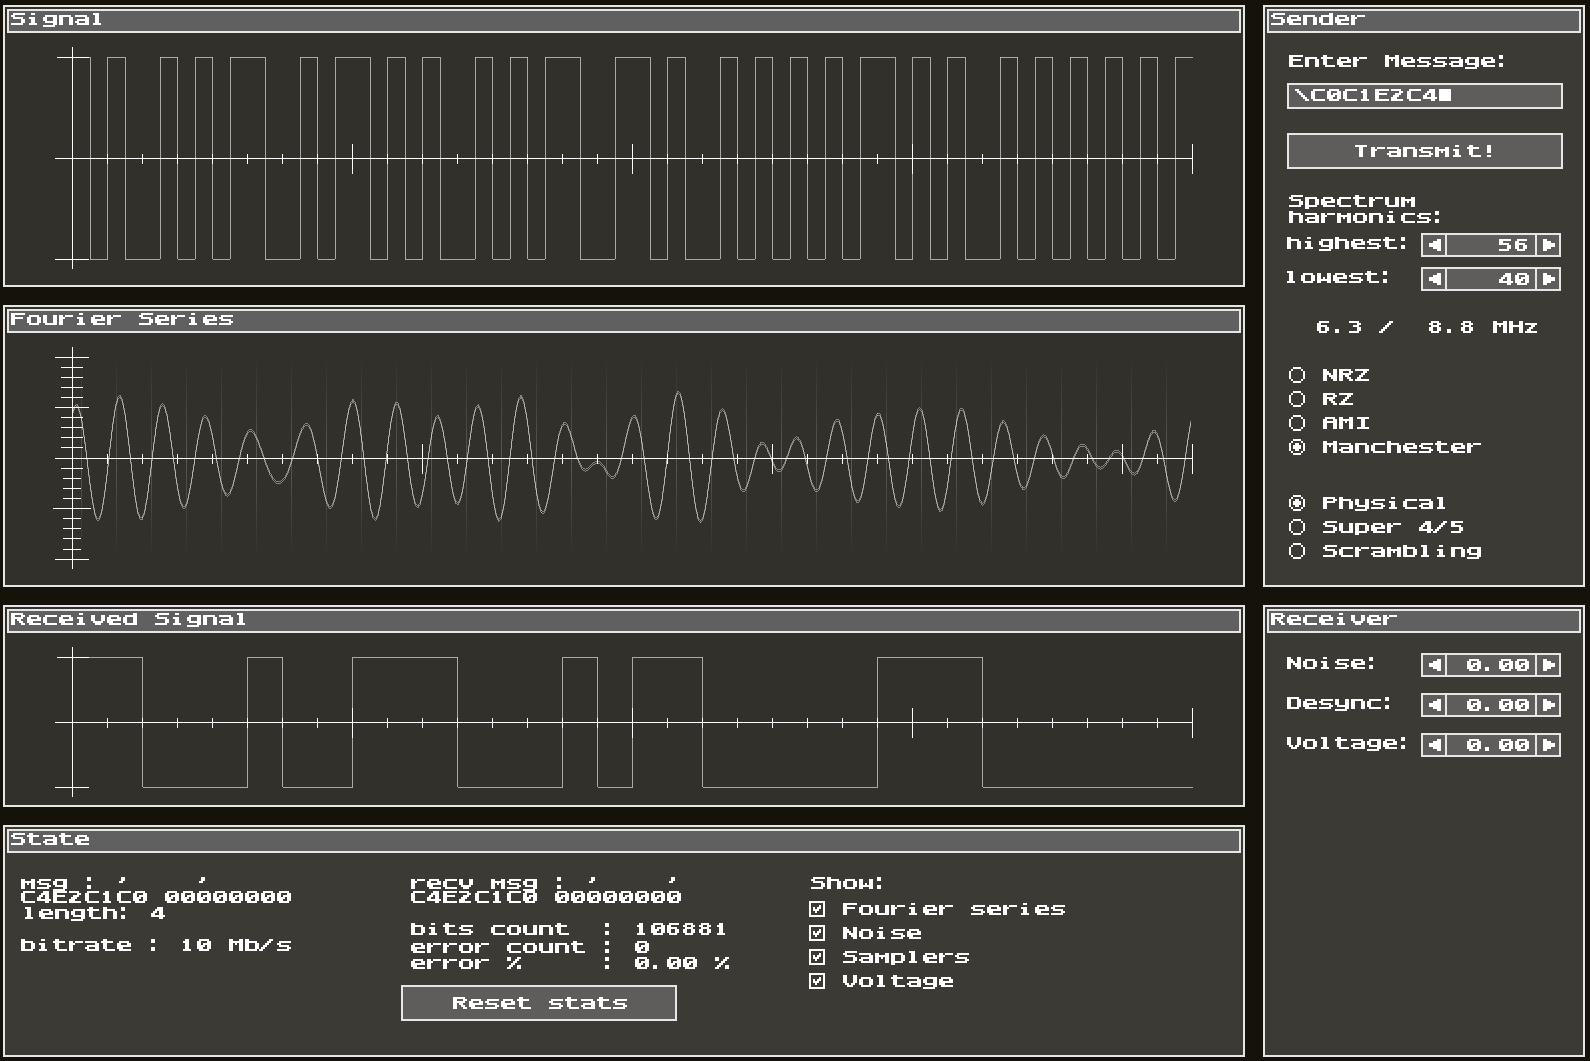
\includegraphics[width=0.95\linewidth]{./data/ideal_m2_min_f.png}
	\cutpic{0.2cm}{11cm}{./data/4_nrz.png.jpg}
	\caption{Процент ошибок для NRZ}
	\vspace{-115pt}
\end{wrapfigure}

Для NRZ при передаче 100000 бит при минимальной ширине полосы пропускания и максимально допустимых уровнях шума, рассинхронизации и граничного напряжения, процент ошибок составил 2.36\%.

\thispagestyle{empty}

\newpage

\subsection{RZ}

\vspace{0.4cm}
\begin{wrapfigure}{r}{0.6\textwidth}
	\centering
	% 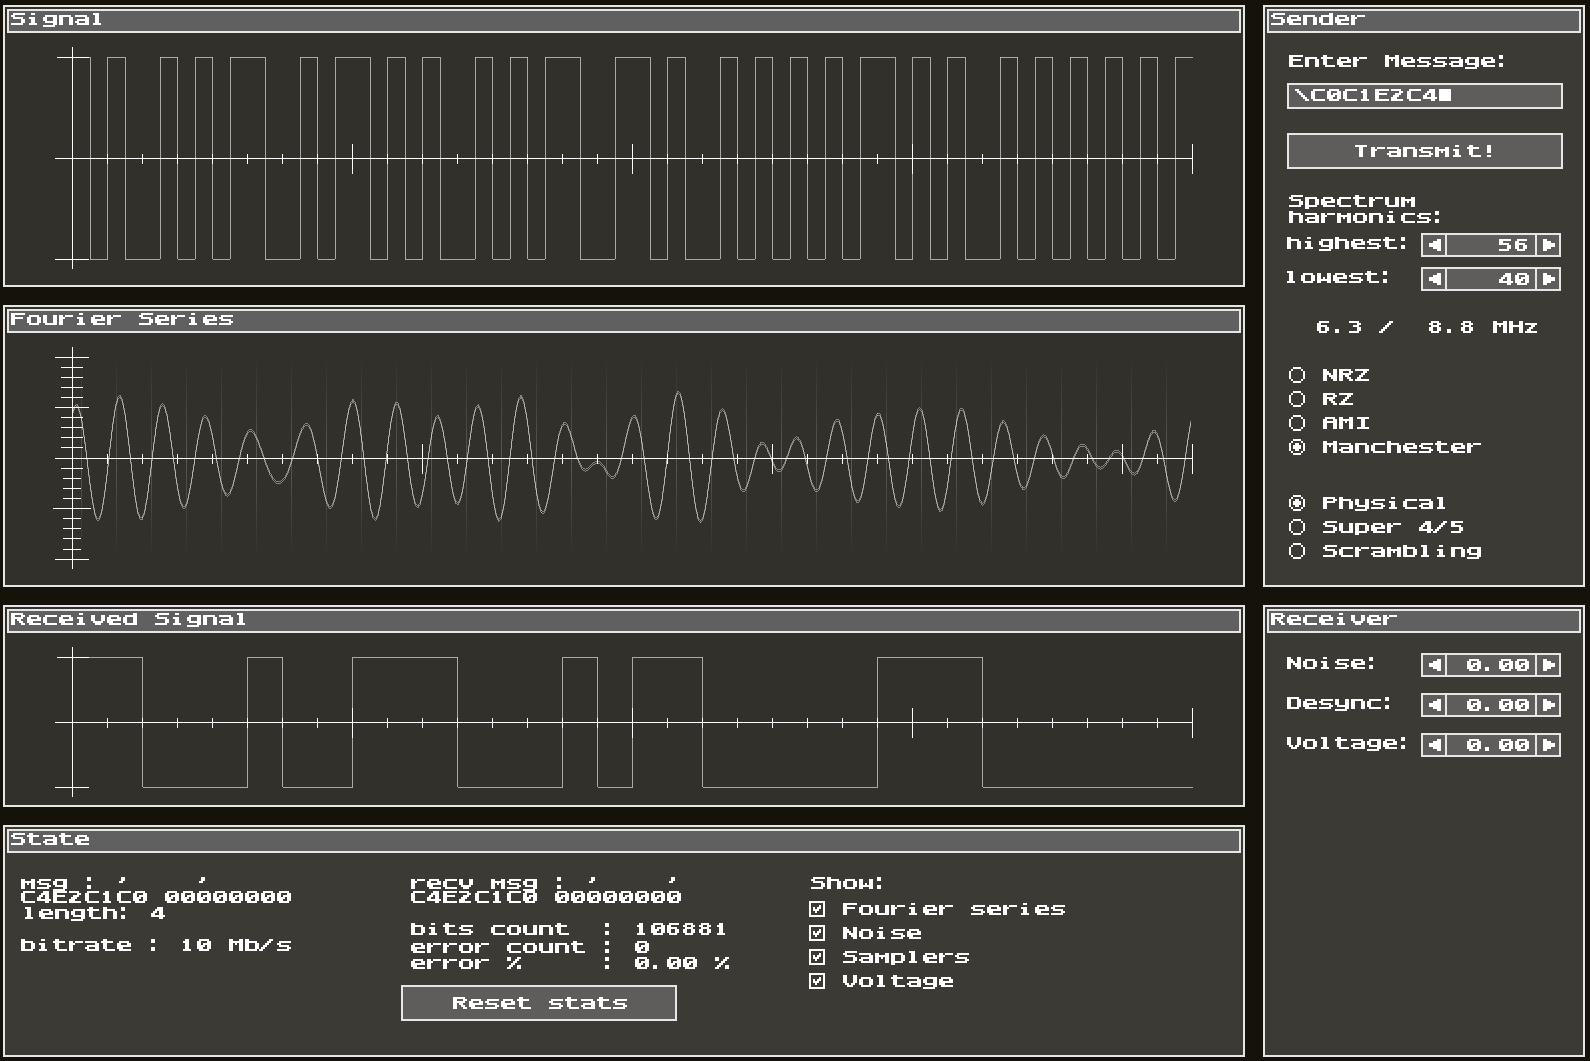
\includegraphics[width=0.95\linewidth]{./data/ideal_m2_min_f.png}
	\cutpic{0.2cm}{11.7cm}{./data/4_rz.png.jpg}
	\caption{Процент ошибок для RZ}
\end{wrapfigure}

Для RZ при передаче 100000 бит при минимальной ширине полосы пропускания и максимально допустимых уровнях шума, рассинхронизации и граничного напряжения, процент ошибок составил 1.2\%.

\subsection{M2}

Для M2 при передаче порядка 100000 бит при минимальной ширине полосы пропускания и максимально допустимых уровнях шума, рассинхронизации и граничного напряжения, процент ошибок составил 0.08\%.

\vspace{0.4cm}
\begin{figure}[H]
	\centering
	% 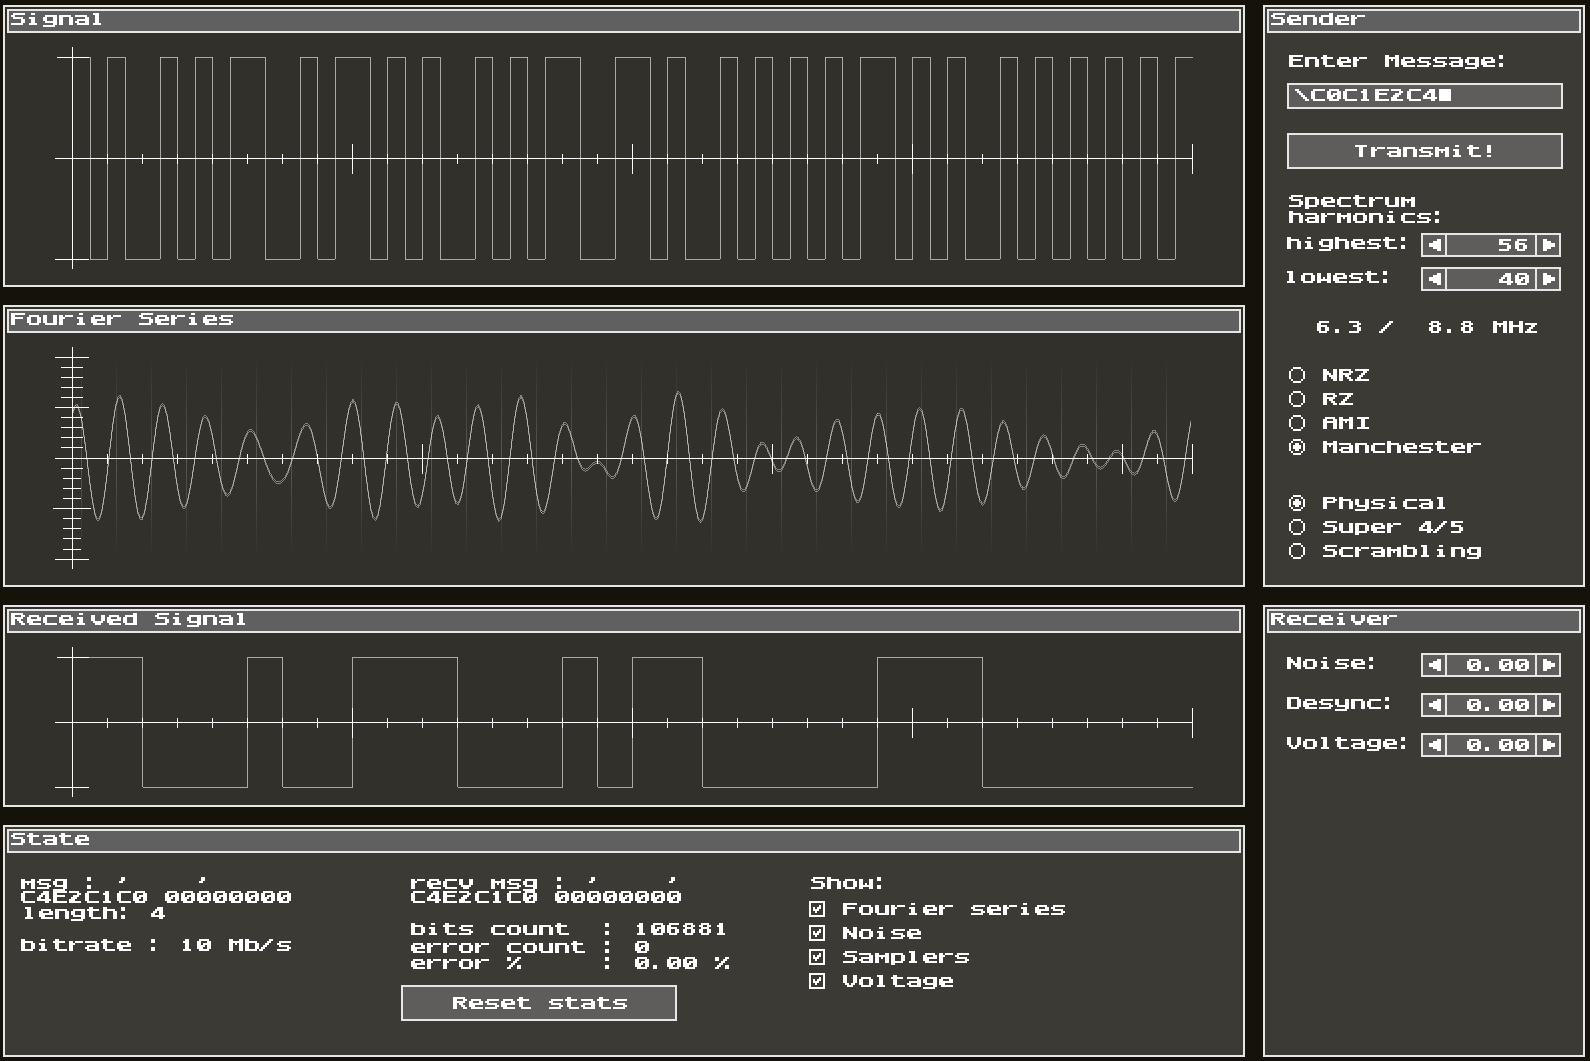
\includegraphics[width=0.95\linewidth]{./data/ideal_m2_min_f.png}
	\cutpic{0.2cm}{16.5cm}{./data/4_m2.png.jpg}
	\caption{Процент ошибок для M2}
\end{figure}

\subsection{NRZ + 4B/5B}

\vspace{0.4cm}
\begin{wrapfigure}{l}{0.7\textwidth}
	\centering
	% 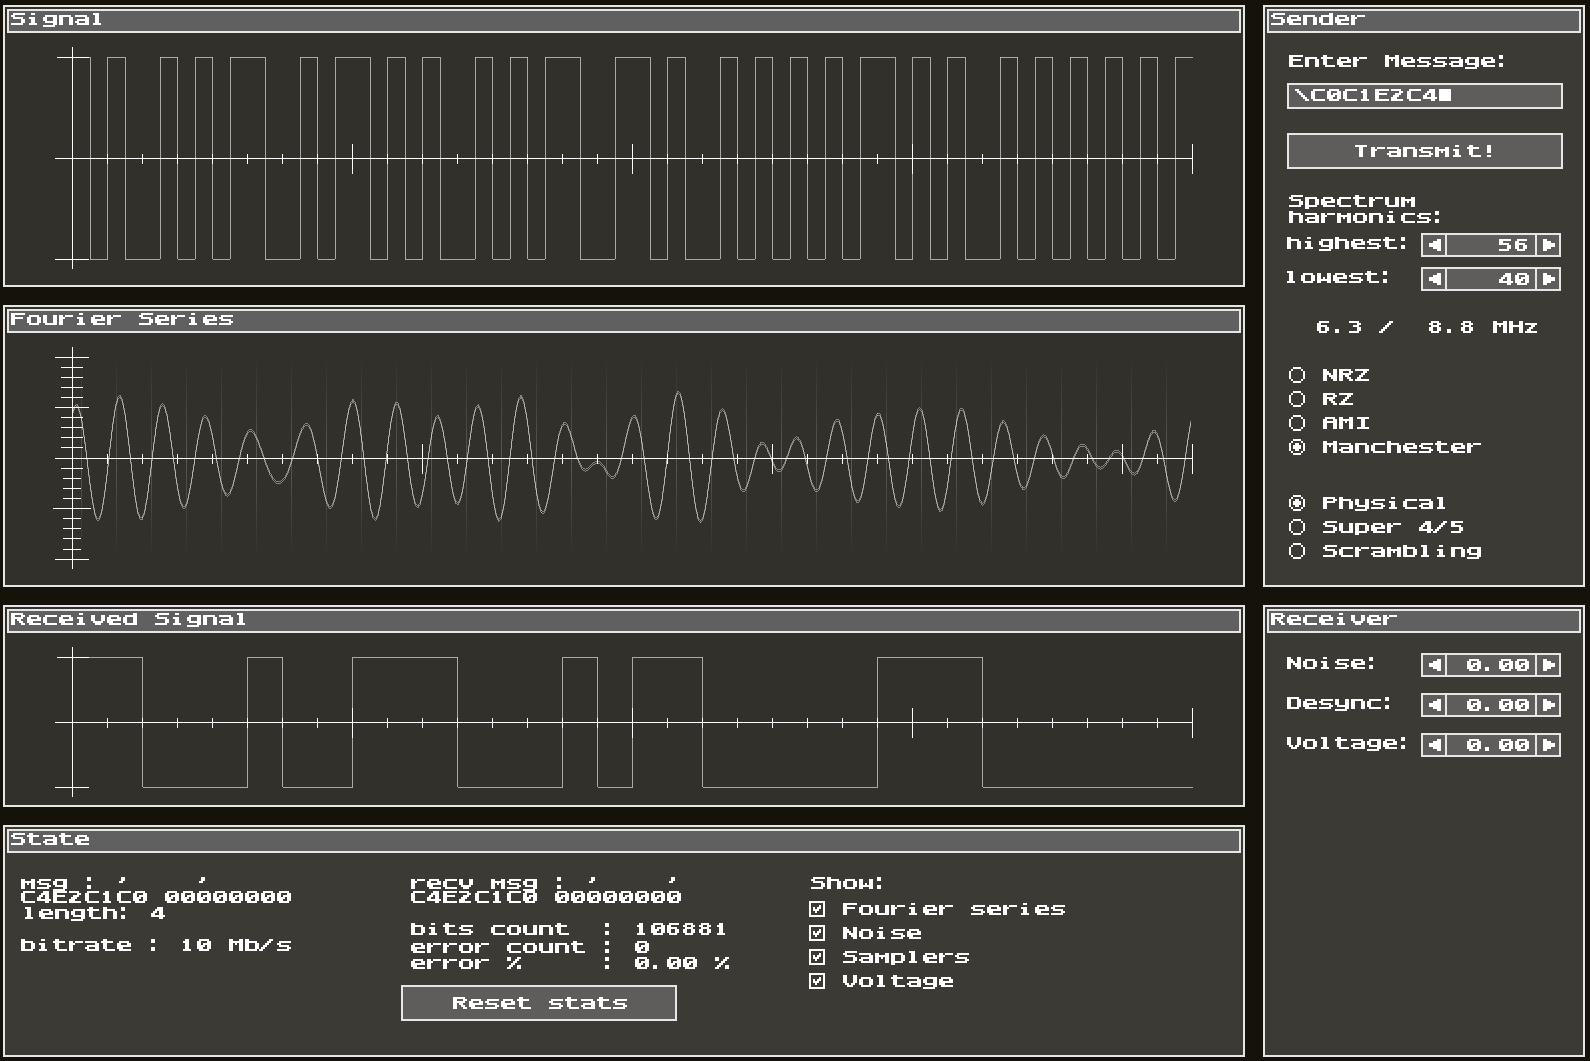
\includegraphics[width=0.95\linewidth]{./data/ideal_m2_min_f.png}
	\cutpic{0.2cm}{12cm}{./data/4_nrz45.png.jpg}
	\caption{Процент ошибок для NRZ + 4B/5B}
    \vspace{-3.7cm}
\end{wrapfigure}

Для NRZ+4B/5B при передаче порядка порядка 100000 бит при минимальной ширине полосы пропускания и максимально допустимых уровнях шума, рассинхронизации и граничного напряжения, процент ошибок составил 1.25\%.

\vspace{3.7cm}
\subsection{NRZ + Scramble}

\vspace{0.4cm}
\begin{wrapfigure}{r}{0.73\textwidth}
	\centering
	% 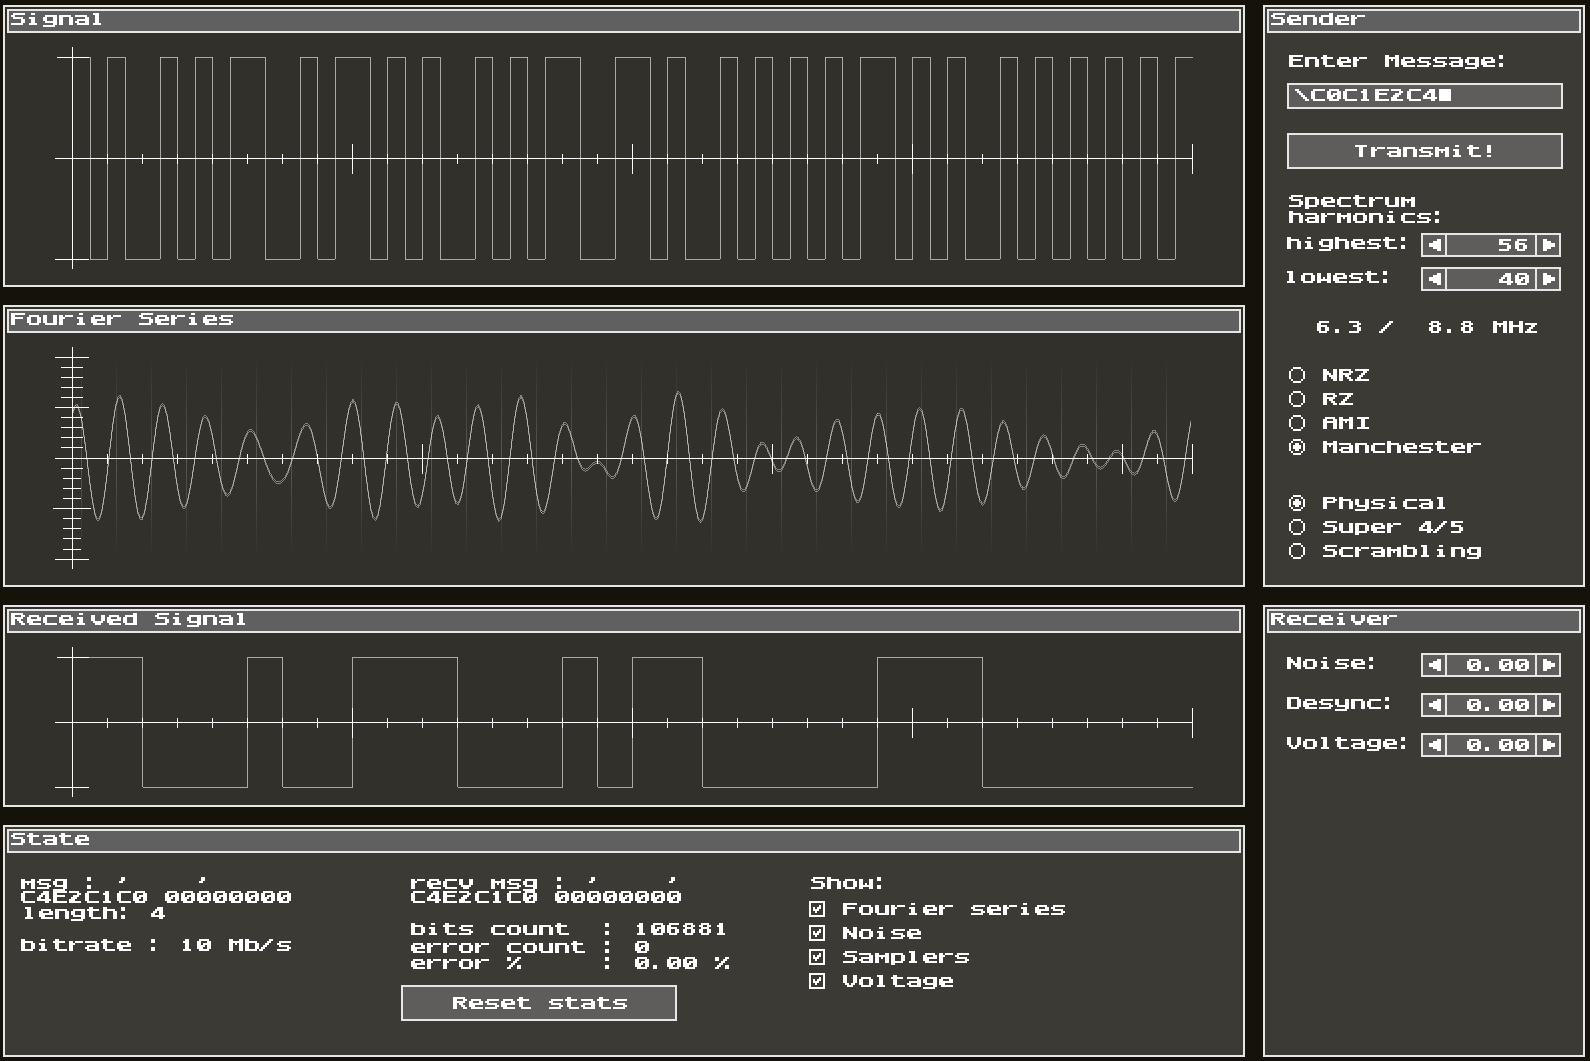
\includegraphics[width=0.95\linewidth]{./data/ideal_m2_min_f.png}
	\cutpic{0.2cm}{14cm}{./data/4_nrzS.png.jpg}
	\caption{Процент ошибок для NRZ + Scramble}
    \vspace{-4.5cm}
\end{wrapfigure}

Для NRZ+Scramble при передаче порядка 100000 бит при минимальной ширине полосы пропускания и максимально допустимых уровнях шума, рассинхронизации и граничного напряжения, процент ошибок составил 2.02\%.

\newpage
\subsection{Выводы}

На данном этапе \underline{лучшим оказался \textbf{Манчестер} (0.08\%)}, что говорит о его устойчивости к различного рода помехам.

Несмотря на то, что на предыдущем этапе NRZ был одним из лучших, в данном тесте он показал худший результат (2.36\%). Такой результат связан с тем, что на предыдущем этапе для него было получены самые высокие уровни помех, и при их совмещение метод оказался сильно подвержен ошибкам.

Такая же картина и у NRZ+Scramble – показав неплохие результаты по отдельности на прошлом этапе, при их совмещении процент ошибок оказался достаточно большим (2.02\%).

Так же объясняется и средний результат RZ и NRZ+4B/5B (1.20\% и 1.25\% соответственно). Так как они показали самые низкие уровни допустимых уровни помех, при их совмещении результат оказался лучше, чем у NRZ и NRZ+Scramble.
